% !TEX root = ./main.tex
% Local-dev build-mode toggle. 1 = handout (\pause overlays collapsed, small
% PDF), 0 = presentation (each \pause becomes a page). CI overrides this via
% latexmk -usepretex, so this line only affects local pdflatex/latexmk runs.
\providecommand{\HANDOUT}{1}
% arena_beamer.sty - shared preamble for all ARENA talk decks.
%
% Loaded BEFORE \documentclass (via plain \input, not \usepackage) so that
% it can decide whether to pass `handout` to beamer based on the \HANDOUT
% toggle. The deck pattern is:
%
%   \providecommand{\HANDOUT}{1}              % 1 = handout, 0 = presentation
%   % arena_beamer.sty - shared preamble for all ARENA talk decks.
%
% Loaded BEFORE \documentclass (via plain \input, not \usepackage) so that
% it can decide whether to pass `handout` to beamer based on the \HANDOUT
% toggle. The deck pattern is:
%
%   \providecommand{\HANDOUT}{1}              % 1 = handout, 0 = presentation
%   % arena_beamer.sty - shared preamble for all ARENA talk decks.
%
% Loaded BEFORE \documentclass (via plain \input, not \usepackage) so that
% it can decide whether to pass `handout` to beamer based on the \HANDOUT
% toggle. The deck pattern is:
%
%   \providecommand{\HANDOUT}{1}              % 1 = handout, 0 = presentation
%   \input{../../arena_beamer.sty}
%   ... deck-local macros ...
%   \begin{document} ... \end{document}
%
% CI overrides the deck's local toggle via latexmk's -usepretex flag, which
% \def's \HANDOUT before main.tex starts. The \providecommand below is a
% safety default if neither the deck nor CI set anything.

\providecommand{\HANDOUT}{1}
\ifnum\HANDOUT=1
  \PassOptionsToClass{handout}{beamer}
\fi
\documentclass[10pt,a4paper]{beamer}

\RequirePackage[latin1]{inputenc}
\RequirePackage{amsmath}
\RequirePackage{amsfonts}
\RequirePackage{amssymb}
\RequirePackage{graphicx}
\RequirePackage{ulem}
\RequirePackage{algorithm2e}
\RequirePackage{algpseudocode}
\RequirePackage{diffcoeff}
\RequirePackage{xcolor}
\RequirePackage{tikz}
\RequirePackage{cancel}
\RequirePackage{pgfplots}
\RequirePackage{background}
\RequirePackage{stmaryrd}
\RequirePackage{subcaption}
\RequirePackage{ifthen}
\RequirePackage{listings}
\RequirePackage{hyperref}

\usetheme{Madrid}

\hypersetup{
    colorlinks=true,
    linkcolor=white,
    filecolor=magenta,
    urlcolor=cyan,
}
\urlstyle{same}

\DeclareMathOperator*{\argmin}{\arg\!\min}
\DeclareMathOperator*{\argmax}{arg\,max}

\usetikzlibrary{calc, fadings, decorations.pathreplacing, automata, positioning, arrows, shapes.geometric, arrows.meta, positioning, fit, backgrounds}

% Generic math/style macros used across decks.
% Anything chapter-specific (state space, reward set, etc.) lives in the
% deck's own main.tex, not here.
\newcommand{\Ex}{\mathbb{E}}
\newcommand{\red}[1]{\textcolor{red}{#1}}
\newcommand{\bth}{{\boldsymbol{\theta}}}

% PyTorch code listing style.
\definecolor{codegreen}{rgb}{0,0.5,0}
\definecolor{codegray}{rgb}{0.4,0.4,0.4}
\definecolor{codepurple}{rgb}{0.55,0.0,0.55}
\definecolor{codeblue}{rgb}{0.0,0.0,0.6}

\lstdefinestyle{pystyle}{
    basicstyle=\ttfamily\scriptsize,
    keywordstyle=\color{codeblue}\bfseries,
    commentstyle=\color{codegreen}\itshape,
    stringstyle=\color{codepurple},
    numberstyle=\tiny\color{codegray},
    breaklines=true,
    showstringspaces=false,
    language=Python,
    morekeywords={self, nn, torch, Tensor},
    columns=fullflexible,
    keepspaces=true,
}
\lstset{style=pystyle}

% Decks set their own \graphicspath after \usepackage{arena_beamer}, but
% default to img/ so plain \includegraphics works without ceremony.
\graphicspath{{img/}}

% Falls back to a labeled placeholder box if the image file isn't present.
% Usage: \imgorplaceholder{0.6\linewidth}{filename-no-ext}{Caption shown if missing}
\newcommand{\imgorplaceholder}[3]{%
    \IfFileExists{img/#2.png}{\includegraphics[width=#1]{#2}}{%
    \IfFileExists{img/#2.jpg}{\includegraphics[width=#1]{#2}}{%
    \IfFileExists{img/#2.pdf}{\includegraphics[width=#1]{#2}}{%
    \IfFileExists{img/#2.svg}{\includegraphics[width=#1]{#2}}{%
        \fbox{\parbox[c][0.45\textheight][c]{#1}{\centering \textit{[image: #3]}\\\scriptsize drop \texttt{img/#2.(png|jpg|pdf)}}}%
    }}}}%
}

\endinput

%   ... deck-local macros ...
%   \begin{document} ... \end{document}
%
% CI overrides the deck's local toggle via latexmk's -usepretex flag, which
% \def's \HANDOUT before main.tex starts. The \providecommand below is a
% safety default if neither the deck nor CI set anything.

\providecommand{\HANDOUT}{1}
\ifnum\HANDOUT=1
  \PassOptionsToClass{handout}{beamer}
\fi
\documentclass[10pt,a4paper]{beamer}

\RequirePackage[latin1]{inputenc}
\RequirePackage{amsmath}
\RequirePackage{amsfonts}
\RequirePackage{amssymb}
\RequirePackage{graphicx}
\RequirePackage{ulem}
\RequirePackage{algorithm2e}
\RequirePackage{algpseudocode}
\RequirePackage{diffcoeff}
\RequirePackage{xcolor}
\RequirePackage{tikz}
\RequirePackage{cancel}
\RequirePackage{pgfplots}
\RequirePackage{background}
\RequirePackage{stmaryrd}
\RequirePackage{subcaption}
\RequirePackage{ifthen}
\RequirePackage{listings}
\RequirePackage{hyperref}

\usetheme{Madrid}

\hypersetup{
    colorlinks=true,
    linkcolor=white,
    filecolor=magenta,
    urlcolor=cyan,
}
\urlstyle{same}

\DeclareMathOperator*{\argmin}{\arg\!\min}
\DeclareMathOperator*{\argmax}{arg\,max}

\usetikzlibrary{calc, fadings, decorations.pathreplacing, automata, positioning, arrows, shapes.geometric, arrows.meta, positioning, fit, backgrounds}

% Generic math/style macros used across decks.
% Anything chapter-specific (state space, reward set, etc.) lives in the
% deck's own main.tex, not here.
\newcommand{\Ex}{\mathbb{E}}
\newcommand{\red}[1]{\textcolor{red}{#1}}
\newcommand{\bth}{{\boldsymbol{\theta}}}

% PyTorch code listing style.
\definecolor{codegreen}{rgb}{0,0.5,0}
\definecolor{codegray}{rgb}{0.4,0.4,0.4}
\definecolor{codepurple}{rgb}{0.55,0.0,0.55}
\definecolor{codeblue}{rgb}{0.0,0.0,0.6}

\lstdefinestyle{pystyle}{
    basicstyle=\ttfamily\scriptsize,
    keywordstyle=\color{codeblue}\bfseries,
    commentstyle=\color{codegreen}\itshape,
    stringstyle=\color{codepurple},
    numberstyle=\tiny\color{codegray},
    breaklines=true,
    showstringspaces=false,
    language=Python,
    morekeywords={self, nn, torch, Tensor},
    columns=fullflexible,
    keepspaces=true,
}
\lstset{style=pystyle}

% Decks set their own \graphicspath after \usepackage{arena_beamer}, but
% default to img/ so plain \includegraphics works without ceremony.
\graphicspath{{img/}}

% Falls back to a labeled placeholder box if the image file isn't present.
% Usage: \imgorplaceholder{0.6\linewidth}{filename-no-ext}{Caption shown if missing}
\newcommand{\imgorplaceholder}[3]{%
    \IfFileExists{img/#2.png}{\includegraphics[width=#1]{#2}}{%
    \IfFileExists{img/#2.jpg}{\includegraphics[width=#1]{#2}}{%
    \IfFileExists{img/#2.pdf}{\includegraphics[width=#1]{#2}}{%
    \IfFileExists{img/#2.svg}{\includegraphics[width=#1]{#2}}{%
        \fbox{\parbox[c][0.45\textheight][c]{#1}{\centering \textit{[image: #3]}\\\scriptsize drop \texttt{img/#2.(png|jpg|pdf)}}}%
    }}}}%
}

\endinput

%   ... deck-local macros ...
%   \begin{document} ... \end{document}
%
% CI overrides the deck's local toggle via latexmk's -usepretex flag, which
% \def's \HANDOUT before main.tex starts. The \providecommand below is a
% safety default if neither the deck nor CI set anything.

\providecommand{\HANDOUT}{1}
\ifnum\HANDOUT=1
  \PassOptionsToClass{handout}{beamer}
\fi
\documentclass[10pt,a4paper]{beamer}

\RequirePackage[latin1]{inputenc}
\RequirePackage{amsmath}
\RequirePackage{amsfonts}
\RequirePackage{amssymb}
\RequirePackage{graphicx}
\RequirePackage{ulem}
\RequirePackage{algorithm2e}
\RequirePackage{algpseudocode}
\RequirePackage{diffcoeff}
\RequirePackage{xcolor}
\RequirePackage{tikz}
\RequirePackage{cancel}
\RequirePackage{pgfplots}
\RequirePackage{background}
\RequirePackage{stmaryrd}
\RequirePackage{subcaption}
\RequirePackage{ifthen}
\RequirePackage{listings}
\RequirePackage{hyperref}

\usetheme{Madrid}

\hypersetup{
    colorlinks=true,
    linkcolor=white,
    filecolor=magenta,
    urlcolor=cyan,
}
\urlstyle{same}

\DeclareMathOperator*{\argmin}{\arg\!\min}
\DeclareMathOperator*{\argmax}{arg\,max}

\usetikzlibrary{calc, fadings, decorations.pathreplacing, automata, positioning, arrows, shapes.geometric, arrows.meta, positioning, fit, backgrounds}

% Generic math/style macros used across decks.
% Anything chapter-specific (state space, reward set, etc.) lives in the
% deck's own main.tex, not here.
\newcommand{\Ex}{\mathbb{E}}
\newcommand{\red}[1]{\textcolor{red}{#1}}
\newcommand{\bth}{{\boldsymbol{\theta}}}

% PyTorch code listing style.
\definecolor{codegreen}{rgb}{0,0.5,0}
\definecolor{codegray}{rgb}{0.4,0.4,0.4}
\definecolor{codepurple}{rgb}{0.55,0.0,0.55}
\definecolor{codeblue}{rgb}{0.0,0.0,0.6}

\lstdefinestyle{pystyle}{
    basicstyle=\ttfamily\scriptsize,
    keywordstyle=\color{codeblue}\bfseries,
    commentstyle=\color{codegreen}\itshape,
    stringstyle=\color{codepurple},
    numberstyle=\tiny\color{codegray},
    breaklines=true,
    showstringspaces=false,
    language=Python,
    morekeywords={self, nn, torch, Tensor},
    columns=fullflexible,
    keepspaces=true,
}
\lstset{style=pystyle}

% Decks set their own \graphicspath after \usepackage{arena_beamer}, but
% default to img/ so plain \includegraphics works without ceremony.
\graphicspath{{img/}}

% Falls back to a labeled placeholder box if the image file isn't present.
% Usage: \imgorplaceholder{0.6\linewidth}{filename-no-ext}{Caption shown if missing}
\newcommand{\imgorplaceholder}[3]{%
    \IfFileExists{img/#2.png}{\includegraphics[width=#1]{#2}}{%
    \IfFileExists{img/#2.jpg}{\includegraphics[width=#1]{#2}}{%
    \IfFileExists{img/#2.pdf}{\includegraphics[width=#1]{#2}}{%
    \IfFileExists{img/#2.svg}{\includegraphics[width=#1]{#2}}{%
        \fbox{\parbox[c][0.45\textheight][c]{#1}{\centering \textit{[image: #3]}\\\scriptsize drop \texttt{img/#2.(png|jpg|pdf)}}}%
    }}}}%
}

\endinput


% Deck-local macros (everything else this deck needs is in arena_beamer.sty).
\newcommand{\green}[1]{\textcolor{green!50!black}{#1}}
\newcommand{\UCB}{\text{UCB}}



\begin{document}

% Title convention: "[<chapter>.<part>] <Topic>". The index page scrapes the
% {{[X.Y] ...}} line; the double braces stop beamer reading the inner [ as a
% short-title arg.
\title[{[2.5] MCTS \& AlphaZero}]
{{[2.5] Monte Carlo Tree Search and AlphaZero}}

 
\author[David Quarel] % (optional, for multiple authors)
{David Quarel}
 
\institute[ARENA] % (optional)
{
  ARENA
}
 
\date[\today] % (optional)
{\today}
 
\frame{\titlepage}

%%%%%%%%%%%%%%%%%%%%%%%%%%%%%%%%%%%%%%%%%%%%%%%%%%%%%%%%%%%%%%%%%%%%%%%%%%%%%%%w
% PART 1: MONTE CARLO TREE SEARCH
%%%%%%%%%%%%%%%%%%%%%%%%%%%%%%%%%%%%%%%%%%%%%%%%%%%%%%%%%%%%%%%%%%%%%%%%%%%%%%%

\section{Monte Carlo Tree Search}

\begin{frame}
	\frametitle{Assumptions}
	
	We consider \textbf{two-player zero-sum games}:
	
	\vspace{0.2cm}
	
	\begin{itemize}
		\item \textbf{Two players:} Taking turns (e.g., White/Black)
		\item \textbf{Zero-sum:} One player's gain = other's loss
		\item \textbf{Deterministic:} No randomness in transitions
		\item \textbf{Perfect information:} Both players see full state
		\item \textbf{Known rules:} Player knows the game dynamics
		\item \textbf{Simulator access:} Can search/simulate future states
	\end{itemize}
	
	\vspace{0.3cm}
	
	\textbf{Payoffs:} $z \in \{+1, 0, -1\}$ (win / draw / loss)
	
	\textbf{No discounting:} $\gamma = 1$ (only final outcome matters)
	
	\vspace{0.3cm}
	
	\small
	Examples: Chess, Go, Checkers, Tic-Tac-Toe, Connect Four
\end{frame}


\begin{frame}
	\frametitle{Classical Approach: Minimax}
	
	\begin{columns}
	\begin{column}{0.45\textwidth}
		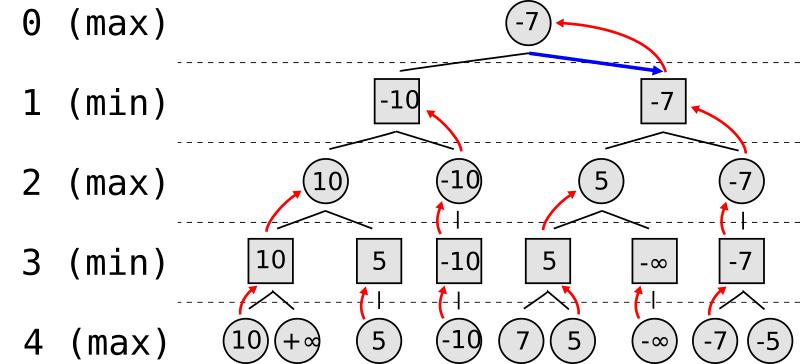
\includegraphics[width=\textwidth]{img/minimax.png}
	\end{column}
	\begin{column}{0.55\textwidth}
		\textbf{Minimax:} Assume opponent plays optimally
		
		\vspace{0.3cm}
		
		\begin{itemize}
			\item MAX nodes: pick child with highest value
			\item MIN nodes: pick child with lowest value
			\item Recursively evaluate to leaves
		\end{itemize}
		
		\vspace{0.3cm}
		
		\textbf{Alpha-beta pruning:} Skip branches that can't affect result
	\end{column}
	\end{columns}
	
\end{frame}


\begin{frame}
	\frametitle{Motivation: Why MCTS?}
	
\begin{itemize}
	\item Minimax + alpha-beta works for Chess ($\approx 35$ moves/position)
	\item Fails for Go ($\approx 250$ moves/position!)
	\begin{itemize}
		\item Branching factor too large
		\item Hard to write evaluation function for non-terminal states
	\end{itemize}
\end{itemize}

\vspace{0.5cm}

\textbf{MCTS Idea:} Don't search exhaustively---\textit{sample} to estimate values.

\vspace{0.3cm}

Build the tree \textit{asymmetrically}, focusing on promising moves.
\end{frame}

\begin{frame}
	\frametitle{MCTS: The Big Picture}
	
	Build search tree incrementally, guided by simulation results.
	
	\vspace{0.5cm}
	
	\textbf{Four phases} (repeated many times):
	\begin{enumerate}
		\item \textbf{Selection} --- Traverse the tree to a leaf node, guided by heuristic
		\item \textbf{Expansion} --- Add child node(s)
		\item \textbf{Simulation} --- Random rollout to terminal state
		\item \textbf{Backpropagation} --- Update statistics along path
	\end{enumerate}
	
	\vspace{0.5cm}
	
	\textbf{Output:} Action with highest visit count from root.
\end{frame}


\begin{frame}
	\frametitle{MCTS: Four Phases}
	
	\begin{center}
		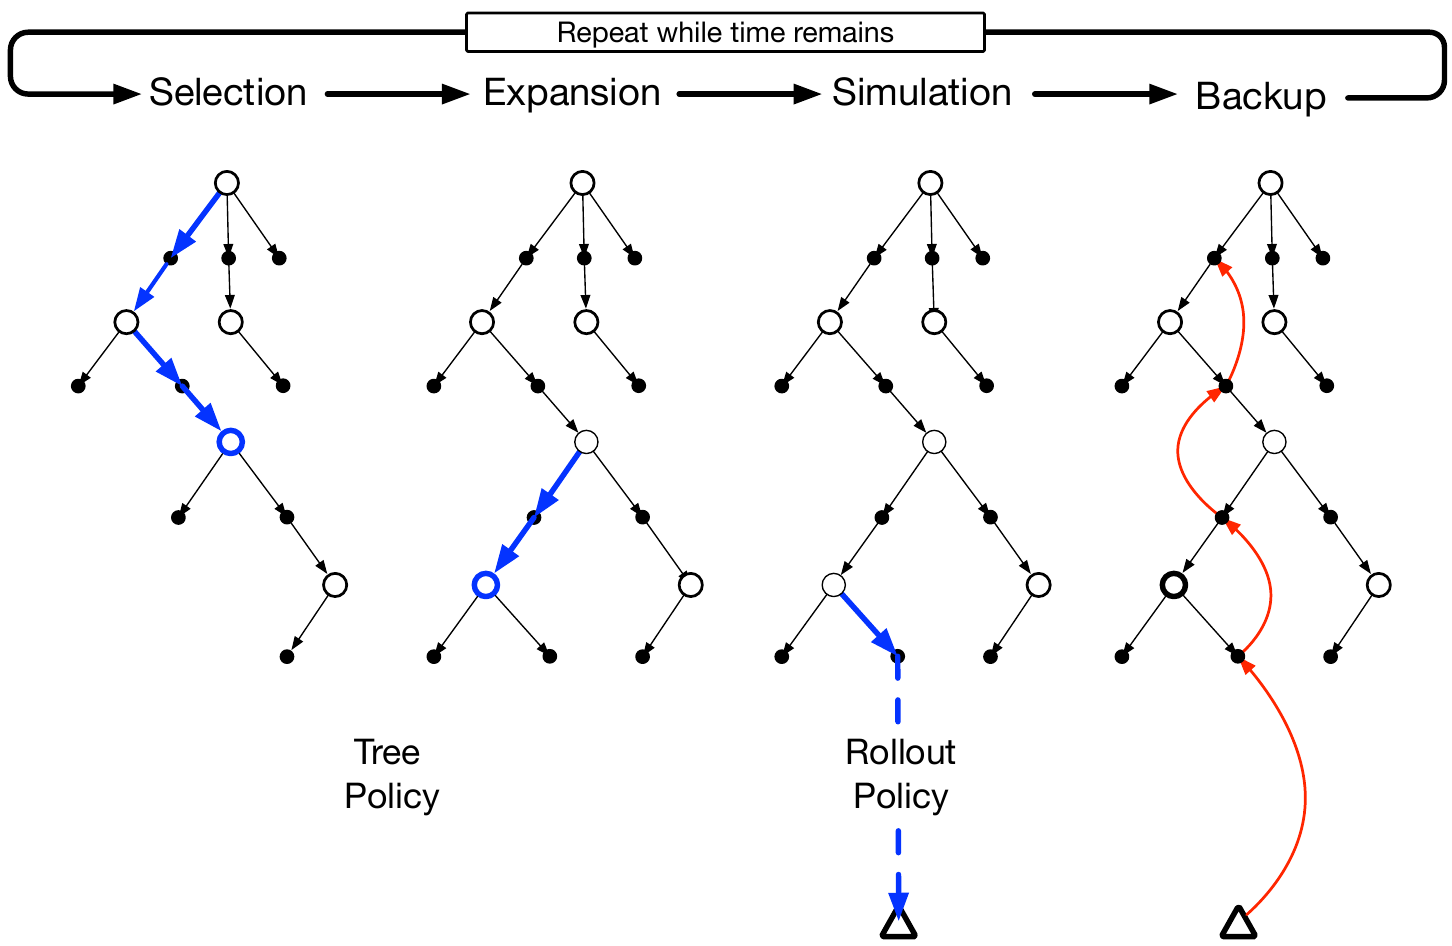
\includegraphics[width=0.95\textwidth]{img/ch25-mcts.png}
	\end{center}
	
	\vspace{0.3cm}
	\small
	\textbf{Selection} $\to$ \textbf{Expansion} $\to$ \textbf{Simulation} $\to$ \textbf{Backpropagation}
	
\end{frame}


\begin{frame}
	\frametitle{Phase 1: Selection (UCT)}
	
	Select child nodes from root to leaf. Balance \textit{exploitation} vs \textit{exploration}.
	
	\begin{block}{UCB1 Formula}
	$$
	\UCB(s, a) = \underbrace{\hat{Q}(s, a)}_{\text{exploit}} + 
	\underbrace{c \sqrt{\frac{\ln N(s)}{N(s, a)}}}_{\text{explore}}
	$$
	\end{block}
	
	\begin{itemize}
		\item $\hat{Q}(s, a)$ = average reward for action $a$ in state $s$
		\item $N(s)$ = total visits to state $s$
		\item $N(s, a)$ = visits to state-action pair $s,a$
		\item \textbf{magic number} $c = \sqrt{2}$ typically
	\end{itemize}
	
	\vspace{0.3cm}
	\small
	\textbf{Theorem:} UCT converges to minimax as simulations $\to \infty$.
\end{frame}


\begin{frame}
	\frametitle{UCB Intuition}
	
	$$
	\UCB(s, a) = \underbrace{\hat{Q}(s, a)}_{\text{exploit}} + 
	\underbrace{c \sqrt{\frac{\ln N(s)}{N(s, a)}}}_{\text{explore}}
	$$
	
	\vspace{0.3cm}
	
	\textbf{Why this formula?}
	
	\begin{itemize}
		\item Estimation error of $\hat{Q}(s,a)$ is $\propto \frac{1}{\sqrt{N(s,a)}}$
		\item Add bonus proportional to uncertainty $\Rightarrow$ explore high-variance actions
		\item $\ln N(s)$ in numerator ensures every action tried infinitely often
	\end{itemize}
	
	\vspace{0.3cm}
	
	\textbf{Behavior:}
	\begin{itemize}
		\item Low $N(s,a)$: Large bonus $\Rightarrow$ explore
		\item High $N(s,a)$: Small bonus $\Rightarrow$ exploit $\hat{Q}$
		\item $\ln$ grows slowly, so exploitation eventually dominates
	\end{itemize}
\end{frame}


\begin{frame}
	\frametitle{Phases 2-4: Expansion, Simulation, Backup}
	
	\textbf{Expansion:} Add one child node (untried action) to the leaf.
	
	\vspace{0.4cm}
	
	\textbf{Simulation (Rollout):} Play randomly to terminal state $\Rightarrow$ reward $z \in \{-1, 0, +1\}$
	
	\vspace{0.4cm}
	
	\textbf{Backpropagation:} Update all nodes on the path:
	\begin{align*}
		N(s) &\leftarrow N(s) + 1 \\
		W(s) &\leftarrow W(s) + z \\
		\hat{Q}(s) &= W(s) / N(s)
	\end{align*}
	
	\vspace{0.3cm}
	\small
	\textbf{Note:} In two-player games, negate $z$ for opponent's nodes.
\end{frame}


\begin{frame}
	\frametitle{MCTS: Pseudocode}
	
	\begin{algorithmic}[1]
		\Function{MCTS}{$s_0$, num\_simulations}
			\State Create root node with state $s_0$
			\For{$i = 1$ to num\_simulations}
				\State $v_l \gets$ \Call{TreePolicy}{root} \Comment{Select + Expand}
				\State $z \gets$ \Call{Rollout}{$s(v_l)$} \Comment{Simulate}
				\State \Call{Backup}{$v_l$, $z$} \Comment{Backprop}
			\EndFor
			\State \Return $\argmax_a N(s_0, a)$
		\EndFunction
	\end{algorithmic}
	
	\vspace{0.5cm}
	
	\small
	\textbf{TreePolicy:} UCB selection $\to$ expand leaf. \quad
	\textbf{Rollout:} Random play to terminal.
\end{frame}


\begin{frame}
	\frametitle{MCTS: Properties}
	
	\textbf{Advantages:}
	\begin{itemize}
		\item \textbf{Anytime:} More iterations = better results
		\item \textbf{Aheuristic:} No hand-crafted evaluation needed
		\item \textbf{Asymmetric:} Focuses on promising branches
		\item \textbf{Parallelizable:} Multiple simulations concurrently
	\end{itemize}
	
	\vspace{0.5cm}
	
	\textbf{Limitations:}
	\begin{itemize}
		\item Random rollouts can be weak
		\item Need a better evaluation function for non-terminal states
	\end{itemize}
\end{frame}


%%%%%%%%%%%%%%%%%%%%%%%%%%%%%%%%%%%%%%%%%%%%%%%%%%%%%%%%%%%%%%%%%%%%%%%%%%%%%%%
% PARALLELIZATION
%%%%%%%%%%%%%%%%%%%%%%%%%%%%%%%%%%%%%%%%%%%%%%%%%%%%%%%%%%%%%%%%%%%%%%%%%%%%%%%

\subsection{Parallelization}

\begin{frame}
	\frametitle{MCTS Parallelization}
	
	MCTS is naturally parallelizable---but \textit{how} matters!
	
	\vspace{0.5cm}
	
	\textbf{Three main strategies:}
	
	\begin{enumerate}
		\item \textbf{Leaf Parallelization}
		\item \textbf{Root Parallelization}
		\item \textbf{Tree Parallelization}
	\end{enumerate}
	
	\vspace{0.5cm}
	
	Trade-off: \textit{Implementation complexity} vs \textit{Speedup efficiency}
\end{frame}


\begin{frame}
	\frametitle{Leaf Parallelization}
	
	\begin{columns}
	\begin{column}{0.5\textwidth}
	\begin{center}
	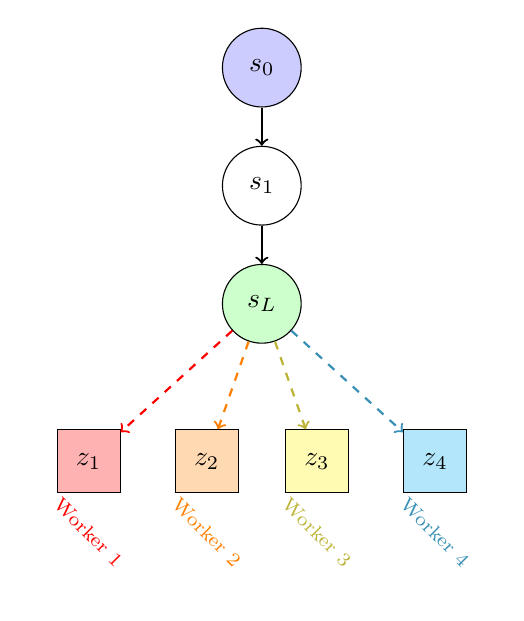
\begin{tikzpicture}[
		every node/.style={circle, draw, minimum size=10mm, font=\normalsize},
		scale=1.0, transform shape
	]
		\node[fill=blue!20] (root) at (0,0) {$s_0$};
		\node (mid) at (0,-1.5) {$s_1$};
		\node[fill=green!20] (leaf) at (0,-3) {$s_L$};
		\draw[->, thick] (root) -- (mid);
		\draw[->, thick] (mid) -- (leaf);
		
		% Multiple rollouts from leaf with worker labels
		\node[rectangle, draw, fill=red!30, minimum size=8mm] (r1) at (-2.2,-5) {$z_1$};
		\node[rectangle, draw, fill=orange!30, minimum size=8mm] (r2) at (-0.7,-5) {$z_2$};
		\node[rectangle, draw, fill=yellow!30, minimum size=8mm] (r3) at (0.7,-5) {$z_3$};
		\node[rectangle, draw, fill=cyan!30, minimum size=8mm] (r4) at (2.2,-5) {$z_4$};
		
		\draw[->, dashed, red, thick] (leaf) -- (r1);
		\draw[->, dashed, orange, thick] (leaf) -- (r2);
		\draw[->, dashed, yellow!70!black, thick] (leaf) -- (r3);
		\draw[->, dashed, cyan!70!black, thick] (leaf) -- (r4);
		
		% Worker labels at 45 degree angle
		\node[draw=none, font=\scriptsize, red, rotate=-45] at (-2.2,-5.9) {Worker 1};
		\node[draw=none, font=\scriptsize, orange, rotate=-45] at (-0.7,-5.9) {Worker 2};
		\node[draw=none, font=\scriptsize, yellow!70!black, rotate=-45] at (0.7,-5.9) {Worker 3};
		\node[draw=none, font=\scriptsize, cyan!70!black, rotate=-45] at (2.2,-5.9) {Worker 4};
	\end{tikzpicture}
	\end{center}
	\end{column}
	
	\begin{column}{0.5\textwidth}
		\textbf{Idea:} Multiple workers run rollouts from the same leaf node in parallel
		
		\vspace{0.5cm}
		
		\green{\checkmark} Simple to implement
		
		\green{\checkmark} No synchronization needed
		
		\vspace{0.3cm}
		
		\red{$\times$} Limited speedup
		
		\red{$\times$} Workers idle during selection
		
		\red{$\times$} All explore same branch
	\end{column}
	\end{columns}
\end{frame}


\begin{frame}
	\frametitle{Root Parallelization}
	
	\textbf{Each worker builds independent tree} --- merge results at the end
	
	\vspace{0.2cm}
	
	\begin{center}
	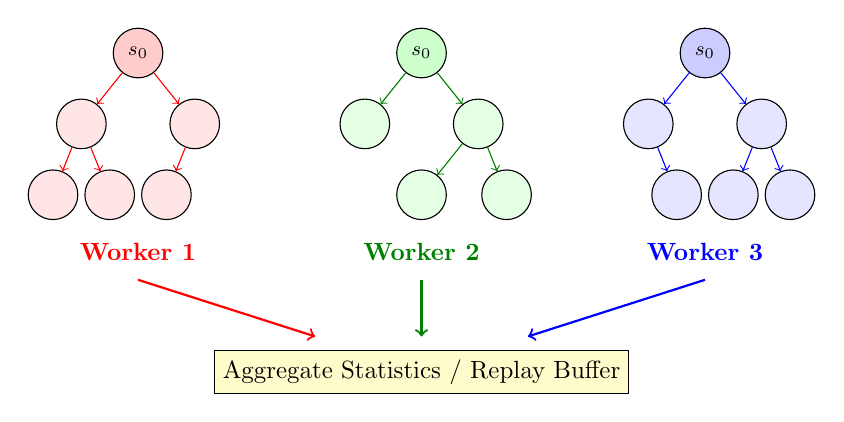
\begin{tikzpicture}[
		every node/.style={circle, draw, minimum size=7mm, font=\footnotesize},
		scale=0.9, transform shape
	]
		% Tree 1 (Red)
		\begin{scope}[xshift=-4cm]
			\node[fill=red!20] (r1) at (0,0) {$s_0$};
			\node[fill=red!10] (c1a) at (-0.8,-1) {};
			\node[fill=red!10] (c1b) at (0.8,-1) {};
			\node[fill=red!10] (c1c) at (-1.2,-2) {};
			\node[fill=red!10] (c1d) at (-0.4,-2) {};
			\node[fill=red!10] (c1e) at (0.4,-2) {};
			\draw[->, red] (r1) -- (c1a);
			\draw[->, red] (r1) -- (c1b);
			\draw[->, red] (c1a) -- (c1c);
			\draw[->, red] (c1a) -- (c1d);
			\draw[->, red] (c1b) -- (c1e);
			\node[draw=none, red, font=\normalsize] at (0,-2.8) {\textbf{Worker 1}};
		\end{scope}
		
		% Tree 2 (Green)
		\begin{scope}[xshift=0cm]
			\node[fill=green!20] (r2) at (0,0) {$s_0$};
			\node[fill=green!10] (c2a) at (-0.8,-1) {};
			\node[fill=green!10] (c2b) at (0.8,-1) {};
			\node[fill=green!10] (c2c) at (0,-2) {};
			\node[fill=green!10] (c2d) at (1.2,-2) {};
			\draw[->, green!50!black] (r2) -- (c2a);
			\draw[->, green!50!black] (r2) -- (c2b);
			\draw[->, green!50!black] (c2b) -- (c2c);
			\draw[->, green!50!black] (c2b) -- (c2d);
			\node[draw=none, green!50!black, font=\normalsize] at (0,-2.8) {\textbf{Worker 2}};
		\end{scope}
		
		% Tree 3 (Blue)
		\begin{scope}[xshift=4cm]
			\node[fill=blue!20] (r3) at (0,0) {$s_0$};
			\node[fill=blue!10] (c3a) at (-0.8,-1) {};
			\node[fill=blue!10] (c3b) at (0.8,-1) {};
			\node[fill=blue!10] (c3c) at (-0.4,-2) {};
			\node[fill=blue!10] (c3d) at (0.4,-2) {};
			\node[fill=blue!10] (c3e) at (1.2,-2) {};
			\draw[->, blue] (r3) -- (c3a);
			\draw[->, blue] (r3) -- (c3b);
			\draw[->, blue] (c3a) -- (c3c);
			\draw[->, blue] (c3b) -- (c3d);
			\draw[->, blue] (c3b) -- (c3e);
			\node[draw=none, blue, font=\normalsize] at (0,-2.8) {\textbf{Worker 3}};
		\end{scope}
		
		% Arrows down to merge
		\draw[->, thick, red] (-4,-3.2) -- (-1.5,-4);
		\draw[->, thick, green!50!black] (0,-3.2) -- (0,-4);
		\draw[->, thick, blue] (4,-3.2) -- (1.5,-4);
		
		% Merge box
		\node[rectangle, draw, fill=yellow!20, minimum width=5cm, minimum height=0.6cm, font=\normalsize] (buffer) at (0,-4.5) {Aggregate Statistics / Replay Buffer};
	\end{tikzpicture}
	\end{center}
	
	\vspace{0.1cm}
	
	\green{\checkmark} No synchronization \quad
	\green{\checkmark} Scales to clusters \quad
	\red{$\times$} Duplicated work across trees
\end{frame}


\begin{frame}
	\frametitle{Tree Parallelization}
	
	\textbf{Multiple workers share one tree} --- different branches simultaneously
	
	\vspace{0.2cm}
	
	\begin{center}
	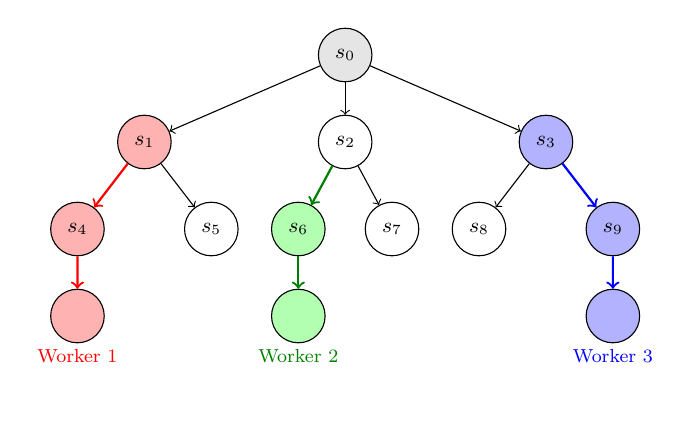
\begin{tikzpicture}[
		every node/.style={circle, draw, minimum size=8mm, font=\small},
		scale=0.85, transform shape
	]
		% Root
		\node[fill=gray!20] (root) at (0,0) {$s_0$};
		
		% Level 1
		\node[fill=red!30] (a) at (-3,-1.3) {$s_1$};
		\node (b) at (0,-1.3) {$s_2$};
		\node[fill=blue!30] (c) at (3,-1.3) {$s_3$};
		
		% Level 2
		\node[fill=red!30] (a1) at (-4,-2.6) {$s_4$};
		\node (a2) at (-2,-2.6) {$s_5$};
		\node[fill=green!30] (b1) at (-0.7,-2.6) {$s_6$};
		\node (b2) at (0.7,-2.6) {$s_7$};
		\node (c1) at (2,-2.6) {$s_8$};
		\node[fill=blue!30] (c2) at (4,-2.6) {$s_9$};
		
		% Level 3 (leaves for some workers)
		\node[fill=red!30] (a1l) at (-4,-3.9) {};
		\node[fill=green!30] (b1l) at (-0.7,-3.9) {};
		\node[fill=blue!30] (c2l) at (4,-3.9) {};
		
		% Edges
		\draw[->] (root) -- (a);
		\draw[->] (root) -- (b);
		\draw[->] (root) -- (c);
		\draw[->, red, thick] (a) -- (a1);
		\draw[->] (a) -- (a2);
		\draw[->, green!50!black, thick] (b) -- (b1);
		\draw[->] (b) -- (b2);
		\draw[->] (c) -- (c1);
		\draw[->, blue, thick] (c) -- (c2);
		\draw[->, red, thick] (a1) -- (a1l);
		\draw[->, green!50!black, thick] (b1) -- (b1l);
		\draw[->, blue, thick] (c2) -- (c2l);
		
		% Worker labels
		\node[draw=none, red, font=\footnotesize] at (-4,-4.5) {Worker 1};
		\node[draw=none, green!50!black, font=\footnotesize] at (-0.7,-4.5) {Worker 2};
		\node[draw=none, blue, font=\footnotesize] at (4,-4.5) {Worker 3};
	\end{tikzpicture}
	\end{center}
	
	\vspace{0.1cm}
	
	\begin{columns}
		\begin{column}{0.5\textwidth}
			\green{\checkmark} No duplicated work---best compute efficiency
		\end{column}
		\begin{column}{0.5\textwidth}
			\red{$\times$} Requires synchronization (locks/atomics)
		\end{column}
	\end{columns}
\end{frame}


\begin{frame}
	\frametitle{Tree Parallelization: Synchronization}
	
	\textbf{Problem:} Multiple threads read/write $N(s), W(s)$ concurrently
	
	\vspace{0.5cm}
	
	\textbf{Option 1: Mutex / Locks}
	\begin{itemize}
		\item Lock node before read/write, unlock after
		\item Simple but high contention at popular nodes (root!)
	\end{itemize}
	
	\vspace{0.3cm}
	
	\textbf{Option 2: Atomic Operations}
	\begin{itemize}
		\item Use atomic increment: \texttt{atomic\_fetch\_add(\&N, 1)}
		\item Lock-free, but limited to simple operations
	\end{itemize}
	
	\vspace{0.3cm}
	
	\textbf{Option 3: Lock-Free with Virtual Loss}
	\begin{itemize}
		\item Atomically add virtual loss during selection
		\item No locks needed---threads naturally spread out
		\item \textbf{AlphaZero uses this approach}
	\end{itemize}
\end{frame}


\begin{frame}
	\frametitle{Virtual Loss: Lock-Free Synchronization}
	
	\textbf{Problem:} Threads all select the same ``best'' node $\Rightarrow$ wasted work
	
	\vspace{0.4cm}
	
	\textbf{Solution:} When thread selects node $s$, \textit{atomically} apply virtual loss:
	$$
	N(s) \xleftarrow{\text{atomic}} N(s) + 1, \quad W(s) \xleftarrow{\text{atomic}} W(s) - 1
	$$
	
	\vspace{0.2cm}
	
	\begin{center}
	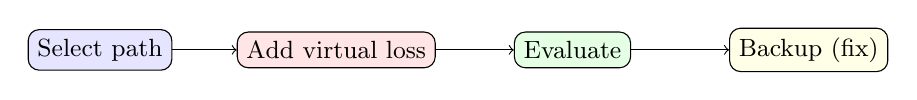
\begin{tikzpicture}[font=\small]
		\node[draw, rounded corners, fill=blue!10] (select) at (0,0) {Select path};
		\node[draw, rounded corners, fill=red!10] (vl) at (3,0) {Add virtual loss};
		\node[draw, rounded corners, fill=green!10] (eval) at (6,0) {Evaluate};
		\node[draw, rounded corners, fill=yellow!10] (backup) at (9,0) {Backup (fix)};
		
		\draw[->] (select) -- (vl);
		\draw[->] (vl) -- (eval);
		\draw[->] (eval) -- (backup);
	\end{tikzpicture}
	\end{center}
	
	\vspace{0.2cm}
	
	\textbf{Effect:} Node looks worse $\Rightarrow$ other threads explore elsewhere
	
	\vspace{0.2cm}
	
	\small
	Mutexes mostly not a problem! Still have to use them in some cases. Atomic ops provide thread safety.
\end{frame}


% \begin{frame}
% 	\frametitle{Parallelization Comparison}
	
% 	\begin{center}
% 	\begin{tabular}{l|c|c|c}
% 		& \textbf{Leaf} & \textbf{Root} & \textbf{Tree} \\
% 		\hline
% 		Complexity & Low & Low & High \\
% 		Synchronization & None & None & Locks \\
% 		Speedup efficiency & Low & Medium & High \\
% 		Memory & $1\times$ & $k\times$ & $1\times$ \\
% 		Distributed & No & Yes & Harder \\
% 	\end{tabular}
% 	\end{center}
	
% 	\vspace{0.5cm}
	
% 	\textbf{AlphaZero uses tree parallelization} with virtual loss.
	
% 	\vspace{0.3cm}
	
% 	\small
% 	Scale: 5000 TPUs for training, 4 TPUs for inference during play.
% \end{frame}


%%%%%%%%%%%%%%%%%%%%%%%%%%%%%%%%%%%%%%%%%%%%%%%%%%%%%%%%%%%%%%%%%%%%%%%%%%%%%%%
% PART 2: ALPHAZERO
%%%%%%%%%%%%%%%%%%%%%%%%%%%%%%%%%%%%%%%%%%%%%%%%%%%%%%%%%%%%%%%%%%%%%%%%%%%%%%%

% \section{AlphaZero}

% \begin{frame}
% 	\frametitle{From AlphaGo to AlphaZero}
	
% 	\begin{tabular}{l|l|l}
% 		\textbf{Version} & \textbf{Year} & \textbf{Key Feature} \\
% 		\hline
% 		AlphaGo Fan & 2015 & Beat European champion \\
% 		AlphaGo Lee & 2016 & Beat Lee Sedol 4-1 \\
% 		AlphaGo Zero & 2017 & \textbf{No human data}, self-play only \\
% 		AlphaZero & 2018 & Chess, Shogi, Go with same algorithm \\
% 	\end{tabular}
	
% 	\vspace{0.8cm}
	
% 	\textbf{Key insight:} Self-play + MCTS + neural networks = superhuman play
	
% 	\vspace{0.3cm}
	
% 	No hand-crafted features, no human games needed.
% \end{frame}


\begin{frame}
	\frametitle{AlphaZero: Key Innovations}
	
	\textbf{Two changes to MCTS:}
	
	\vspace{0.5cm}
	
	\textbf{1. Neural network replaces rollouts}
	\begin{itemize}
		\item Directly estimate value $v$ --- no random simulation
	\end{itemize}
	
	\vspace{0.5cm}
	
	\textbf{2. Learned prior guides search}
	\begin{itemize}
		\item Policy $\mathbf{p}$ focuses on promising moves
	\end{itemize}
	
	\vspace{0.5cm}
	
	$\Rightarrow$ Far fewer simulations needed (800 vs 10,000+)
\end{frame}


\begin{frame}
	\frametitle{Neural Network Architecture}
	
	Single network with two heads:
	$$
	f_\bth(s) = \big(P_\bth(\cdot|s), \, \hat{V}_\bth(s)\big)
	$$
	
	\vspace{0.5cm}
	
	\begin{tabular}{l|l}
		\textbf{Policy head} $P_\bth(\cdot|s)$ & Prob. distribution over actions \\
		& $\Rightarrow$ guides MCTS selection \\
		\hline
		\textbf{Value head} $\hat{V}_\bth(s) \in [-1,+1]$ & Estimated win probability \\
		& $\Rightarrow$ replaces rollouts \\
	\end{tabular}
	
	\vspace{0.5cm}
	
	\textbf{Architecture:} ResNet with two linear heads
\end{frame}


\begin{frame}
	\frametitle{AlphaZero MCTS}
	
	\begin{center}
		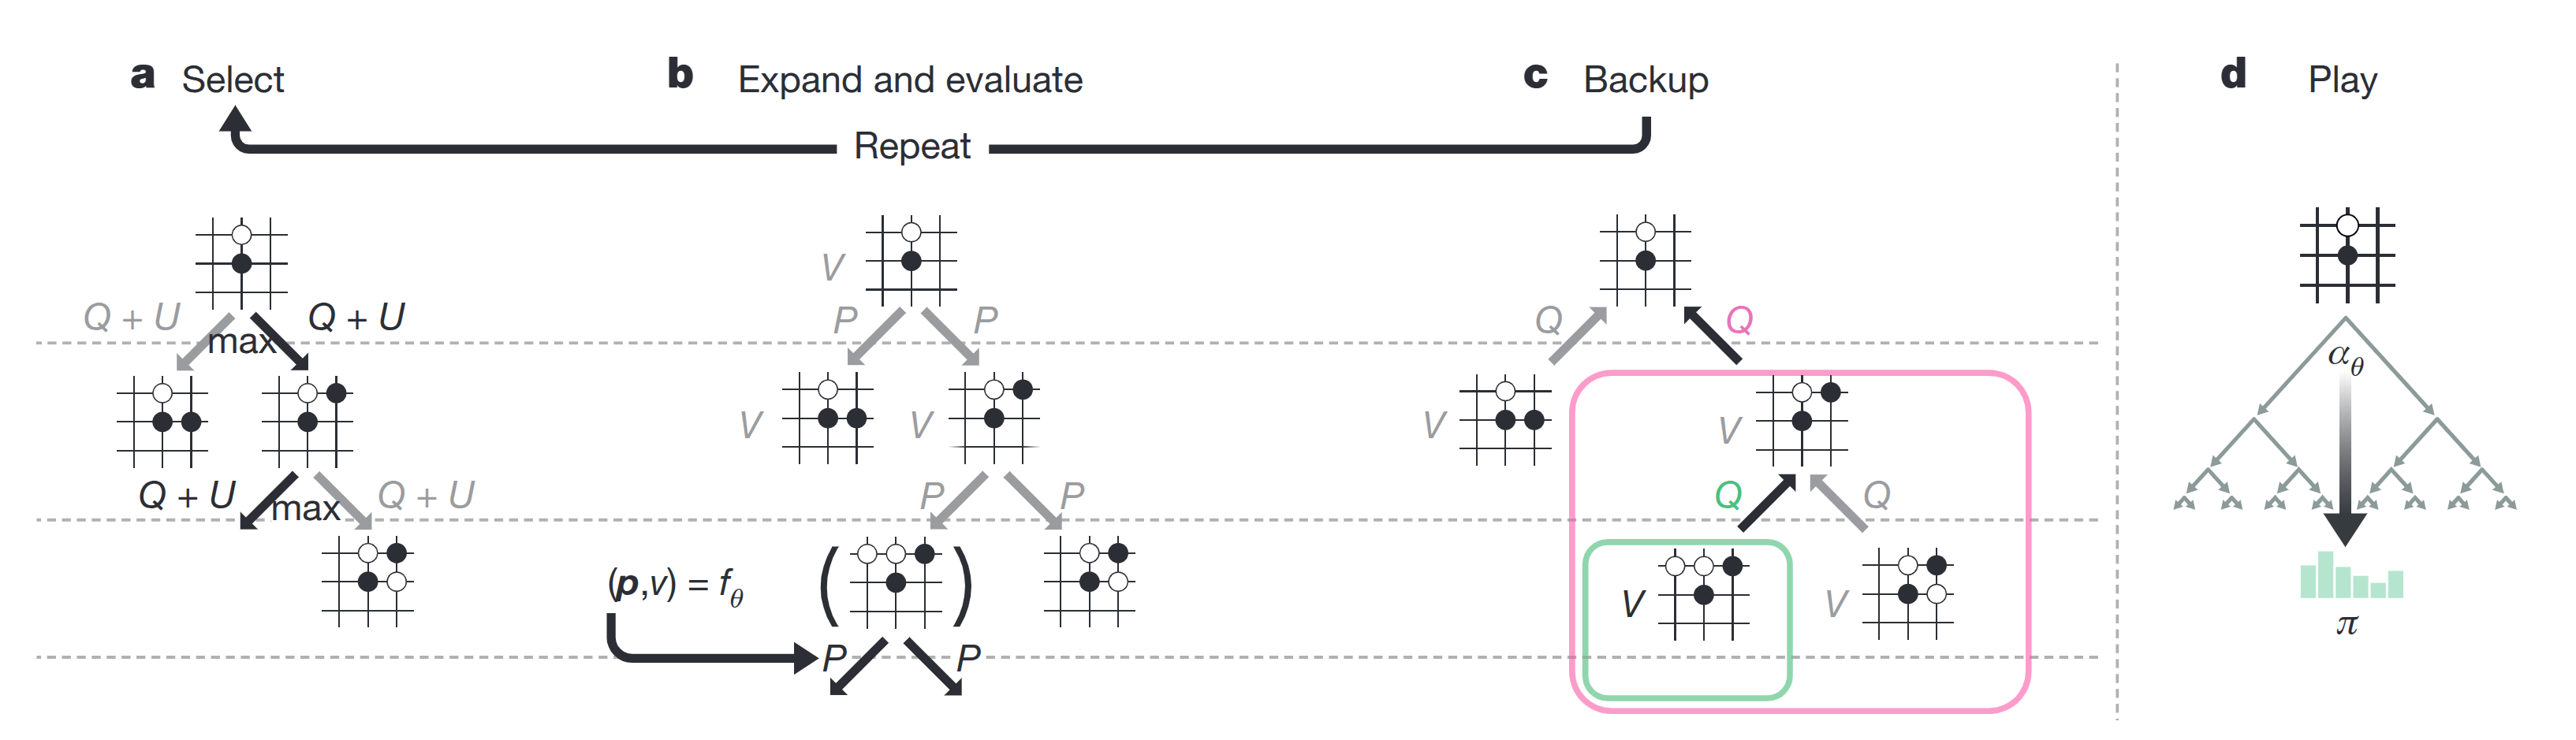
\includegraphics[width=1\linewidth]{img/alpha_zero.png}
	\end{center}
	
	\vspace{0.2cm}
	
	\textbf{Key difference:} No simulation/rollout---$\hat{V}_\bth(s)$ provides backup signal directly.
\end{frame}


\begin{frame}
	\frametitle{PUCT: Selection with Prior}
	
	AlphaZero uses \textbf{PUCT} instead of UCB:
	
	\begin{block}{PUCT Tree Policy}
	$$
	a^* = \argmax_a \left[ Q(s, a) + c_{\text{puct}} \cdot \red{P_\bth(a|s)} \cdot \frac{\sqrt{1+N(s)}}{1 + N(s, a)} \right]
	$$
	\end{block}
	
	\vspace{0.3cm}
	
	\textbf{Key difference:} Prior $\red{P_\bth(a|s)}$ from network weights exploration
	
	\vspace{0.3cm}
	
	\begin{itemize}
		\item Initially: explore actions network likes ($P_\bth(a|s)$ high)
		\item Later: $Q(s,a)$ dominates (exploitation)
		\item Search can override prior if data disagrees
	\end{itemize}
	
	\vspace{0.3cm}
	
	\textbf{Result:} Network provides intuition, MCTS refines it.
\end{frame}


\begin{frame}
	\frametitle{MCTS Policy: $\boldsymbol{\pi}$}
	
	After running MCTS, we extract an \textbf{improved policy} from visit counts:
	
	$$
	\pi(a|s) = \frac{N(s,a)^{1/\tau}}{\sum_{a'} N(s,a')^{1/\tau}}
	$$
	
	\vspace{0.3cm}
	
	\textbf{Temperature $\tau$} controls exploration:
	\begin{itemize}
		\item $\tau = 1$: $\pi(a|s) \propto N(s,a)$ (proportional to visits)
		\item $\tau \to 0$: $\pi(a|s) \to \mathbf{1}[a = \argmax_{a'} N(s,a')]$ (deterministic)
	\end{itemize}
	
	\vspace{0.3cm}
	
	\textbf{Key insight:} $\boldsymbol{\pi}$ is \textit{better} than network's prior $P_\bth(\cdot|s)$!
	\begin{itemize}
		\item MCTS refines the policy through search
		\item Use $\boldsymbol{\pi}$ as training target to improve the network
	\end{itemize}
\end{frame}


\begin{frame}
	\frametitle{AlphaZero: The Loss Function}
	
	The neural network $f_\bth(s) = \big(P_\bth(\cdot|s), \hat{V}_\bth(s)\big)$ is trained to minimize:
	
	\begin{block}{AlphaZero Loss}
	$$
	L(\bth) = \underbrace{(z - \hat{V}_\bth)^2}_{\text{value loss}} + 
	\underbrace{(-\boldsymbol{\pi}^T \log \mathbf{p}_\bth)}_{\text{policy loss}} + 
	\underbrace{c \|\bth\|^2}_{\text{L2 reg.}}
	$$
	\end{block}
	
	\vspace{0.3cm}
	
	\textbf{Training data from self-play:}
	\begin{itemize}
		\item $\boldsymbol{\pi}$ = MCTS visit distribution (target policy)
		\item $z \in \{-1, +1\}$ = game outcome (target value)
	\end{itemize}
	
\end{frame}


\begin{frame}
	\frametitle{Loss Function: Components}
	
	\begin{block}{AlphaZero Loss (Expanded)}
	$$
	L(\bth) = (z - \hat{V}_\bth(s))^2 - \sum_{a \in \mathcal{A}} \pi(a|s) \log P_\bth(a|s) + c \|\bth\|^2
	$$
	\end{block}
	
	\vspace{0.3cm}
	
	\textbf{Value Loss} (MSE): learn to predict game outcome
	$$
	L_v = (z - \hat{V}_\bth(s))^2
	$$
	
	\textbf{Policy Loss} (Cross-entropy): distill MCTS into network
	$$
	L_\pi = -\boldsymbol{\pi}^T \log \mathbf{p}_\bth = -\sum_{a \in \mathcal{A}} \pi(a|s) \log P_\bth(a|s)
	$$
	
	\textbf{L2 Regularization}: prevent overfitting
	$$
	L_{\text{reg}} = c \|\bth\|^2
	$$
\end{frame}


\begin{frame}
	\frametitle{Policy Loss: Why Cross-Entropy?}
	
	We want the network policy $\mathbf{p}_\bth$ to match MCTS policy $\boldsymbol{\pi}$:
	$$
	L_\pi = D_{\text{KL}}(\boldsymbol{\pi} \| \mathbf{p}_\bth) = \sum_{a} \pi(a) \log \frac{\pi(a)}{P_\bth(a)}
	$$
	
	\vspace{0.3cm}
	
	Expanding and differentiating:
	\begin{align*}
	\nabla_\bth L_\pi &= \nabla_\bth \left[ \underbrace{\sum_a \pi(a) \log \pi(a)}_{-H(\boldsymbol{\pi}), \text{ const. w.r.t. } \bth} - \sum_a \pi(a) \log P_\bth(a) \right] \\[0.3cm]
	&= -\nabla_\bth \sum_a \pi(a) \log P_\bth(a)
	\end{align*}
	
	\vspace{0.3cm}
	
	$\Rightarrow$ Minimizing KL $\Leftrightarrow$ minimizing \textbf{cross-entropy}:
	$$
	L_\pi = -\sum_{a} \pi(a|s) \log P_\bth(a|s)
	$$
\end{frame}


\begin{frame}
	\frametitle{Policy Improvement via Distillation}
	
	\textbf{Key insight:} MCTS improves the policy!
	
	\vspace{0.5cm}
	
	\begin{center}
	\begin{tikzpicture}[node distance=2.5cm, every node/.style={font=\small}]
		\node[draw, rounded corners] (net) {Network $P_\bth$};
		\node[draw, rounded corners, right of=net] (mcts) {MCTS};
		\node[draw, rounded corners, right of=mcts] (pi) {$\boldsymbol{\pi}$ (better!)};
		\node[draw, rounded corners, below of=mcts] (train) {Train};
		
		\draw[->] (net) -- (mcts);
		\draw[->] (mcts) -- (pi);
		\draw[->] (pi) -- (train);
		\draw[->] (train) -- (net);
	\end{tikzpicture}
	\end{center}
	
	\vspace{0.3cm}
	
	Better network $\to$ better MCTS $\to$ better targets $\to$ better network...
\end{frame}


\begin{frame}
	\frametitle{Self-Play Training Loop}
	
	\begin{algorithmic}[1]
		\State Initialize network $f_\bth$ randomly
		\Loop
			\State \textbf{Self-play:} Run MCTS, collect $(s, \boldsymbol{\pi}, z)$
			\State \textbf{Train:} Minimize $L(\bth)$ on minibatch
		\EndLoop
	\end{algorithmic}

	\vspace{0.3cm}

	\begin{block}{What is the value target $z$?}
		Each self-play game is played out to the end. \textbf{$z$ is simply that
		game's terminal value} ($+1$/$0$/$-1$), assigned to \textit{every} state $s$
		the game passed through---not just the final position. So the critic
		$\hat{V}_\bth(s)$ is regressed onto the eventual outcome (a Monte-Carlo
		estimate), which is well-defined even when $s$ is non-terminal.
	\end{block}

	\vspace{0.3cm}

	\textbf{Temperature $\tau$} controls move selection: $\pi(a) \propto N(s, a)^{1/\tau}$
	
	\vspace{0.3cm}
	
	\begin{itemize}
		\item $\tau = 1$: Sample proportional to visits (exploration)
		\item $\tau \to 0$: Pick most visited (exploitation)
	\end{itemize}
	
	\vspace{0.3cm}
	
	\small
	AlphaZero: $\tau=1$ for first 30 moves, then $\tau \to 0$.
\end{frame}


% \begin{frame}
% 	\frametitle{AlphaZero vs Traditional MCTS}
	
% 	\begin{center}
% 	\begin{tabular}{l|c|c}
% 		& \textbf{MCTS} & \textbf{AlphaZero} \\
% 		\hline
% 		Selection & UCB & PUCT + prior \\
% 		Evaluation & Random rollout & Network $v$ \\
% 		Prior & Uniform & Network $\mathbf{p}$ \\
% 		Simulations & 1000s & 100s \\
% 	\end{tabular}
% 	\end{center}
	
% 	\vspace{0.5cm}
	
% 	\textbf{Synergy:} Network provides fast intuition, MCTS refines it.
% \end{frame}


% \begin{frame}
% 	\frametitle{Results}
	
% 	\begin{center}
% 	\begin{tabular}{l|l|l}
% 		\textbf{Game} & \textbf{Opponent} & \textbf{Result} \\
% 		\hline
% 		Chess & Stockfish 8 & 28W-72D-0L \\
% 		Go & AlphaGo Lee & 100W-0L \\
% 		Shogi & Elmo & 90W-8D-2L \\
% 	\end{tabular}
% 	\end{center}
	
% 	\vspace{0.5cm}
	
% 	\textbf{Training:} 4 hours (Chess), 40 days (Go) on TPUs
	
% 	\textbf{Inference:} 800 MCTS simulations per move
	
% 	\vspace{0.3cm}
	
% 	No human games, no hand-crafted features---just self-play.
% \end{frame}


\begin{frame}
	\frametitle{Summary}
	
	\textbf{MCTS:} Select $\to$ Expand $\to$ Simulate $\to$ Backup
	
	\vspace{0.3cm}
	
	\textbf{AlphaZero:} Replace simulation with neural network $f_\bth(s) = \big(P_\bth(\cdot|s), \hat{V}_\bth(s)\big)$
	
	\vspace{0.5cm}
	
	\textbf{Loss:}
	$$
	L = \underbrace{(z-\hat{V}_\bth)^2}_{\text{value}} + \underbrace{(-\boldsymbol{\pi}^T \log \mathbf{p}_\bth)}_{\text{policy}} + \underbrace{c\|\bth\|^2}_{\text{reg}}
	$$
	
	\vspace{0.5cm}
	
	\textbf{Parallelization:} Leaf, Root, or Tree (with virtual loss)
\end{frame}


\begin{frame}
	\frametitle{References}
	
	\begin{itemize}
		\item Sutton \& Barto, \textit{Reinforcement Learning: An Introduction}, Chapter 8.11
		\url{http://incompleteideas.net/book/the-book-2nd.html}
		
		\item Silver et al., \textit{Mastering the game of Go with deep neural networks and tree search} (Nature, 2016)
		\url{https://www.nature.com/articles/nature16961}
		
		\item Silver et al., \textit{Mastering the game of Go without human knowledge} (Nature, 2017)
		\url{https://www.nature.com/articles/nature24270}
		
		\item Silver et al., \textit{A general reinforcement learning algorithm that masters chess, shogi, and Go through self-play} (Science, 2018)
		\url{https://www.science.org/doi/10.1126/science.aar6404}
		
		\item Browne et al., \textit{A Survey of Monte Carlo Tree Search Methods} (2012)
		\url{https://ieeexplore.ieee.org/document/6145622}
	\end{itemize}
\end{frame}



\end{document}

